\newif\ifglobal

%%%%%%%%%%%%%%%%%%%%%%%
%%% Compile to view %%%
%%%%%%%%%%%%%%%%%%%%%%%

%%%%%%%%%%%%%%%%%%%%%%%%%%%%%%%%%%%%%%%%%%%%%%%%%%%
%%% Readme:                                     %%%
%%% https://www.overleaf.com/read/bwdjvfjksvjy/ %%%
%%%%%%%%%%%%%%%%%%%%%%%%%%%%%%%%%%%%%%%%%%%%%%%%%%%

% >>> M?: marks a module setting number or important notice

% >>> M4: Set {./relative-path} to external files for this module <<<
\def \modulefiles {./24-ETHERNETMAC}
% To add an external file, use:
% (Replace '---' with actual filename)
% '\input{\modulefiles/tables/---.tex}' for tables
% '\includegraphics{\modulefiles/figures/---}' for figures
% '\subfile{\modulefiles/---}' for register files


% >>> M1: This module is in global project? <<<
% 'YES' - uncomment; 'NO' - comment out
\globaltrue

\ifglobal
    \documentclass[main\_\_CN.tex]{subfiles}

\else
    % Font "FandolSong-Regular" used by ctex does not have GSUB table.
    % It causes warnings that do not affect compilation and can be ignored.
    \PassOptionsToPackage{quiet}{fontspec}

    \documentclass[openany, 10pt]{book}

    % >>> M2: In ./00-shared/preamble-trm-module, also find
    %         settings for visibility of todo notes, watermark <<<
    \usepackage{preamble-trm-module}

    % Enable Chinese typesetting
    \usepackage{ctex}

    % >>> M3: Temporary labels in Chinese
    %         you can add your own labels there <<<
    \myexternaldocument{./00-shared/temp-labels-cn}

\fi %\ifglobal


\setcounter{secnumdepth}{4}


% >>> M5: If this module needs any updates in
% './00-shared/preamble-trm-module.sty'
% (include additional package, etc.), contact your module PM
% or create the file './00-shared/changelog.tex' make the
% necessary updates yourself and document them in this file <<<

% Make text left-aligned and allow latex to break pages naturally, comment out for full justification
\raggedright
\raggedbottom


\begin{document}


% Sets language into which pre-defined bits of text are translated
\selectlanguage{chinese}
\setchineseformatting


% Do not delete this block
\ifglobal
% Add the following front matter if
% this module is outside of global project
\else
    \InputIfFileExists{readme}{}{}
    \listoftodos
    {\let\clearpage\relax \listofdonetodos}
    \tableofcontents
    %\listoftables
    %\listoffigures
\fi


%%%%%%%%%%%%%%%%%%%%%%%%%
%%% TRM Module Begins %%%
%%%%%%%%%%%%%%%%%%%%%%%%%

\hypertarget{ethernetmac}{}
\chapter{以太网介质访问控制器 (EMAC)}
\label{mod:ethernetmac}

\section{概述}
{\bfseries Ethernet 主要特性}\\
借助外部以太网物理层 (Ethernet PHY)，ESP32 可以通过以太网介质访问控制 (Ethernet MAC) 按照 IEEE 802.3 标准发送和接收数据。详见图 \ref{Figure:ehternet_mac_overview}。以太网是当前应用最普遍的局域网 (LAN) 和广域网 (WAN) 进行数据传播的网络协议。

\begin{figure}[H]
    \centering
    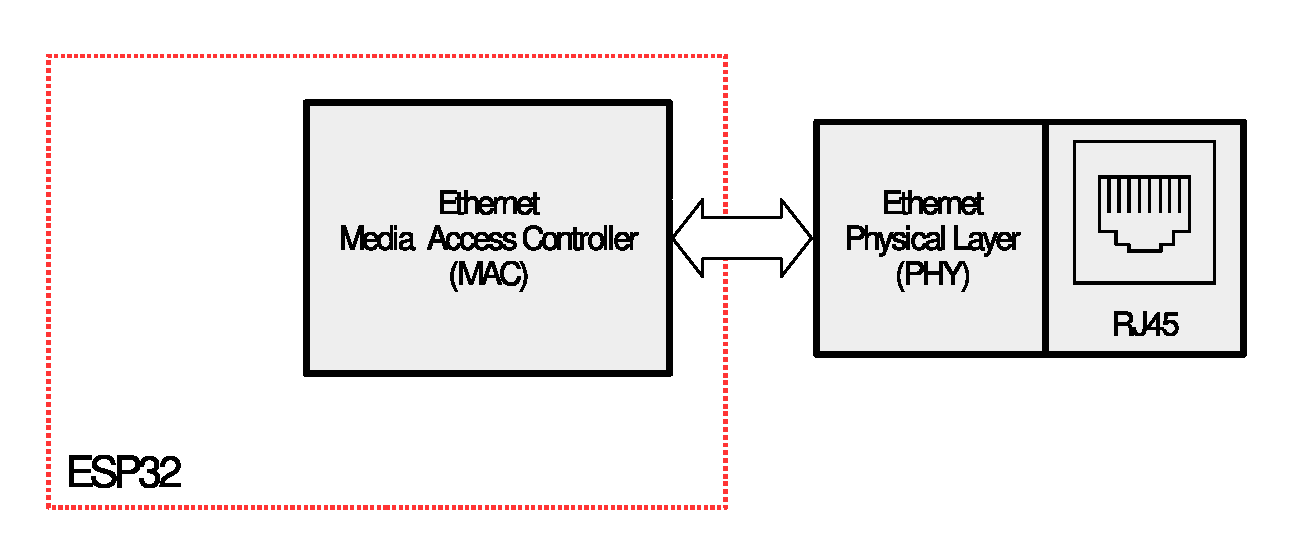
\includegraphics[width=0.7\textwidth]{./24-ETHERNETMAC/figures/ehternet_mac_overview}
    \caption{Ethernet MAC 功能概述}
    \label{Figure:ehternet_mac_overview}
\end{figure}

ESP32 以太网 MAC 符合以下标准：
\begin{itemize}
		\item IEEE 802.3-2002，用于以太网 MAC。
	\item 符合 IEEE 802.3 规范工业标准接口：介质独立接口 (MII) 和简化介质独立接口 (RMII)。
\end{itemize}
{\bfseries MAC 层特性}
\begin{itemize}
	\item 支持外部 PHY 接口实现 10/100 Mbit/s 数据传输速率
	\item 可通过符合 IEEE802.3 的 MII 接口和 RMII 接口与外部快速以太网 PHY 进行通信
	\item 支持全双工和半双工模式 \begin{itemize}
    	\item 支持适用于半双工模式的 CSMA/CD 协议
		\item 支持适用于全双工模式的 IEEE 802.3x 流量控制
		\item 全双工模式时可以将接收的暂停控制帧转发到用户应用程序
		\item 半双工模式时提供背压流量控制
		\item 全双工操作中如果流量控制输入信号消失，将自动发送暂停时间为零的暂停帧
		\end{itemize}
	\item 报头和帧起始数据 (SFD) 在发送路径中插入、在接收路径中删除
	\item 可逐帧控制 CRC 和 pad 自动生成
	\item 如果数据为达到最小帧长度，则自动添加 pad
	\item 可编程帧长度，支持高达 16 KB 的巨型帧
	\item 可编程帧间隔 (IFG)（40-96 位时间，以 8 为步长）
	\item 支持多种灵活的地址过滤模式:
		 \begin{itemize}
    	\item 高达 8 个 48 位完美地址过滤器，对每个字节进行掩码操作
		\item 高达 8 个 48 位 SA 地址比较检查，对每个字节进行掩码操作
		\item 可传送所有多播地址帧
		\item 支持混合模式，因此可传送所有帧，无需为网络监视进行过滤
		\item 传送所有传入数据包时（每次过滤时）均附有一份状态报告    \end{itemize}
	\item 为发送和接收数据包分别返回 32 位状态
	\item 为应用程序提供单独的发送、接收和控制接口
	\item 使用 MDIO 接口配置和管理 PHY 设备
	\item 在接收功能中支持对接收到的由以太网帧封装的 IPv4 和 TCP 数据包进行校验和卸载
	\item 在接收功能中支持检查 IPv4 头校验和以及在 IPv4/IPv6 数据包中封装的 TCP、UDP 或 ICMP 校验和
	\item 两组 FIFO：一个具有可编程阈值功能的 2 KB 发送 FIFO 和一个具有可配置阈值（默认为 64 个字节）功能的 2 KB 接收 FIFO
	\item 接收 FIFO 进行多帧存储时，在 EOF 传输后，通过向接收 FIFO 插入接收状态矢量，从而使得接收 FIFO 无需存储这些帧的接收状态
	\item 在存储转发模式下，可以在接收时过滤所有的错误帧，但不将这些错误帧转发给应用程序
	\item 可以转发过小的好帧
	\item 为接收 FIFO 中由于溢出丢失或损坏的帧生成脉冲，借此支持数据统计
	\item 向 MAC 内核发送数据时支持存储转发机制
	\item 发送时处理冲突帧的自动重新发送（符合一定条件，详见 \ref{section:Retransmission During a Collision}）
	\item 丢弃延迟冲突、过度冲突、过度延迟和下溢条件下的帧
	\item 通过软件控制刷新 Tx FIFO
	\item 计算 IPv4 头校验和与 TCP、UDP 或 ICMP 校验和并将其插入在存储转发模式下发送的帧中
\end{itemize}
\newpage {\bfseries Ethernet 结构框图}

Ethernet 结构框图如图 \ref{Figure:Ethernet_block_diagram} 所示。\\
\begin{figure}[H]
    \centering
    
\includegraphics[width=0.8\textwidth]{./24-ETHERNETMAC/figures/Ethernet_block_diagram}
    \caption{Ethernet 功能框图}
    \label{Figure:Ethernet_block_diagram}
\end{figure}

Ethernet MAC 层主要包括 EMAC\_CORE，EMAC\_MTL (MAC Transition Layer)，EMAC\_DMA (Direct Memory Access) 三层以及 MAC 层的配置寄存器模块，
它们分别有 Rx 和 Tx 两个方向，在芯片内部通过 AHB 和 APB 总线和系统相连接，在芯片外部通过 MII 和 RMII 接口和外部的 PHY 进行通信，最终实现以太网的功能。

\section{EMAC\_CORE}
MAC 支持许多兼容 PHY 芯片的接口。复位后 PHY 接口只能选一次。MAC 使用 MAC 发送接口 (MTI)，MAC 接收接口 (MRI) 和 MAC 控制接口 (MCI) 与应用侧（DMA 侧）进行通信。

\subsection{传输操作}
当 MTL 应用程序推送数据并且 SOF（帧起始）信号拉高时，启动发送操作。当检测到 SOF 信号时，MAC 接收数据并开始发送到 RMII 或 MII。应用程序启动传输之后将帧数据发送到 RMII 或 MII 所需的时间取决于延迟因素，如 IFG 延迟，发送报头或 SFD（起始帧分隔符）的时间以及半双工的任何回退延迟模式。在此之前，通过拉低数据就绪信号，MAC 不接收从 MTL 接收到的数据。

在 EOF（帧结束）发送到 MAC 之后，MAC 完成正常传输，并将传输状态 (Transmit Status) 提供给 MTL。如果在传输过程中（在半双工模式下）发生正常的冲突，则 MAC 使 MTL 的发送状态有效。 然后它接受并删除所有剩下的数据，直到接收到下一个 SOF。在传输状态中检测到 MAC 发出的重试请求时，MTL 模块应该从 SOF 开始重传相同的帧。

如果 MTL 不能在传输期间连续提供数据，则 MAC 会发出下溢状态。在从 MTL 正常传输帧的过程中，如果 MAC 接收到一个 SOF 而没有得到前一帧的 EOF，则忽略该 SOF，并将该新帧视为前一帧的延续。

\subsubsection{发送流量控制 }
在全双工模式下，当发送流量控制使能位（Flow Control Register 中的 TFE/Transmit Flow Control 位）置 1 时，MAC 将生成暂停帧并根据需要发送暂停帧。暂停帧与计算出的 CRC 附加在一起并发送。可以通过两种方式启动暂停帧的生成。

当应用程序将 Flow Control Register 中的 FCB (Flow Control Busy) 位置 1 或接收 FIFO 已满时，将发送暂停帧。

\begin{itemize}
\item 如果应用程序已通过将 Flow Control Register 寄存器中的 FCB 位置 1 来请求流量控制，则 MAC 将生成并发送单个 暂停帧。生成的帧中的暂停时间值为 Flow Control Register 中编程的暂停时间值。 要在先前发送的暂停帧中指定的时间之前延长或结束暂停时间，应用程序必须以适当的值编程暂停时间值（Flow Control Register 中的 PT/Pause Time），然后请求 另一次暂停帧发送。
\item 如果接收 FIFO 填满时应用程序已请求流量控制，则 MAC 将生成并发送暂停帧。生成的帧中的暂停时间值为 Flow Control Register中编程的暂停时间值。如果在此暂停时间结束前，接收 FIFO 在可配置的时隙数（Flow Control Register 中的 PLT (Pause Low Threshold) 位）期间保持填满状态，将发送第二个暂停帧。只要接收 FIFO 保持填满状态，该过程将一直重复下去。如果在采样时间之前不再满足此条件，MAC 将发送一个暂停时间为零的暂停帧，向远程端表明接收缓冲区已准备好接收新数据帧。
\end{itemize}
\subsubsection{冲突期间的重新发送}\label{section:Retransmission During a Collision}
在半双工模式下，向 MAC 传输帧时，可能在 MAC 线接口上发生冲突事件。MAC 甚至会在接收到帧结束之前就给出状态来指示重试。然后将使能重新发送并再次将帧从 FIFO 中弹出。当超过 96 个字节弹向 MAC 内核后，FIFO 控制器将释放该空间，使 DMA 可推入更多数据。这意味着超过阈值后或 MAC 内核指示延迟冲突事件时，无法重新发送。

由于碰撞，Tx FIFO 下溢，载波丢失，jabber 超时，无载波，过度延迟或迟冲突，MAC 发送器都可能会中止帧的传输。 当帧传输由于冲突而中止时，MAC 请求重发帧。

\subsection{接收操作}
当 MAC 在 RMII 或 MII 上检测到 SFD 时启动接收操作。在继续处理帧之前，MAC 剥去前导码和 SFD。检查报头字段的过滤和用于验证帧的 CRC 的 FCS 字段。 接收的帧存储在缓冲器中，直到执行地址过滤。如果帧未通过地址过滤，则帧丢弃在 MAC 中。

MAC 接收的帧将推入 Rx FIFO。此 FIFO 的状态一旦超过配置的接收阈值（Operation Mode 寄存器中的 Receive Threshold Control/RTC 位），并通知给 DMA，这样 DMA 可向 AHB 接口发起预配置的突发传输。

在默认直通模式下，当 FIFO 接收到 64 个字节（通过 Operation Mode 寄存器中的 Receive Threshold Control/RTC 位配置）或完整的数据包时，数据将弹出，其可用性将通知给 DMA。DMA 向 AHB 接口发起传输后，数据传输将从 FIFO 持续 进行，直到传输完整个数据包。完成帧 EOF 的传输后，状态字将弹出并发送到 DMA 控制器。

在 Rx FIFO 存储转发模式（通过 Operation Mode 寄存器中的 Receive Store and Forward/RSF 位配置），这样只会读出有效帧并将其转发到应用程序。在直通模式下，某些错误帧不会被丢弃，因为在帧结束时才接收到错误状态，而此时帧数据已从 FIFO 读出。

\subsubsection{接收协议}
接收模块接收到包之后，去除接收的帧的报头和 SFD。检测到 SFD 后，MAC 开始向接收 FIFO 发送以太网帧数据，从 SFD 后面的第一个字节（目标地址）开始发送。

如果接收的帧长度/类型字段小于 0x600 并且为 MAC 使能了自动去除 CRC/pad 选项，则 MAC 将向接收 FIFO 发送帧数据（数据量不超过长度/类型字段中指定的数量），然后开始丢弃字节（包括 FCS 字段）。如果长度/类型字段大于或等于 0x600，则不管配置的自动 CRC 去除选项的值如何，MAC 都会向 Rx FIFO 发送所有接收到的 以太网帧数据。默认情况下，使能 MAC 看门狗定时器，即，超过 2048 个字节（DA+SA+LT+数据+pad+FCS）帧会被切断。可通过对 MAC 配置寄存器中的 看门狗禁止 (WD/Watchdog Disable) 位编程来禁止此功能。但是，即使禁止看门狗定时器，仍将切断大于 16 KB 的帧并给出看门狗超时状态。

\subsubsection{接收帧控制器 }
如果复位 MAC 帧过滤寄存器中的 RA (Receive All) 位，则 MAC 将根据目标/源地址执行帧过滤。如果应用程序决定不接收任何不良帧，如矮帧、CRC 错误帧等，则仍需要执行另一等级的过滤。检测到过滤失败时，帧将被丢弃且不会传输到应用程序。当过滤参数动态改变时，如果 (DA-SA) 过滤失败，则剩余的帧将被丢弃并且接收状态字将立即更新（零帧长度位、CRC 错误位和矮帧错误位将置 1），指示过滤失败。

\subsubsection{接收流量控制 }
MAC 将检测接收暂停帧并暂停帧发送，暂停时间为接收的暂停帧内指定的延迟（仅限全双工模式）。可通过 Flow Control Register 中的 (Receive Flow Control Enable/RFCE) 位使能或禁止暂停帧检测功能。使能接收流量控制后，将开始监视接收帧的目标地址是否与控制帧的多播地址 (0x0180 C200 0001) 匹配。如果检测到匹配 （接收的帧的目标地址与保留的控制帧的目标地址匹配），MAC 将根据 Frame Filter Register 中的 (Pass Control Frames/PCF) 位来决定是否将接收的控制帧传输应用程序。

MAC 还将对接收控制帧的类型、操作码和暂停定时器字段进行解码。如果状态的字节计数指示 64 个字节，并且不存在任何 CRC 错误，则 MAC 发送器将暂停任何数据帧的 发送，暂停时间为解码的暂停时间值乘以时隙（对于 10/100 Mbit/s 模式，均为 64 字节）。同时，如果检测到另一个零暂停时间值的暂停帧，MAC 将复位暂停时间 并管理新的暂停请求。

如果接收的控制帧与类型字段 (0x8808)、操作码 (0x00001) 以及字节长度（64 字节）均不匹配，或存在 CRC 错误，则 MAC 不会暂停。

如果暂停帧具有多播目标地址，MAC 将根据地址匹配来过滤帧。

对于具有单播目标地址的暂停帧，MAC 将根据 DA 是否与 MAC 地址 0 寄存器的内容匹配以及 Flow Control Register 中的 UPFD (Unicast Pause Frame Detect) 位是否置 1（检测具有单播目标地址的暂停帧）来进行过滤。PCF 寄存器位（Frame Filter Register 中的 Pass Control Frames 位 [7:6]）可对控制帧的过滤以及地址过滤进行控制。

\subsubsection{接收多帧的操作处理}
由于接收数据后状态立即可用，因此只要 FIFO 未满，就可以向其中存储帧。
\subsubsection{错误处理 }
如果在从 MAC 接收 EOF 数据之前 Rx FIFO 已满，则将产生上溢并丢弃整个帧。由于上溢， 状态位 (RDESO[11]) 将指示这是一个部分帧。如果使用 Operation Mode Register 中的 FTF (Flush Transmit FIFO) 和 FUGF (Forward Undersized Good Frames) 位使能相应功能，Rx FIFO 可过滤错误帧和过小帧。如果将接收 FIFO 配置为在存储转发模式下工作，则可过滤并丢弃所有错误帧。

在直通模式下，如果在从 Rx FIFO 读取帧的 SOF 时，该帧的状态和长度可用，则可 丢弃整个错误帧。DMA 可通过使能接收帧清空位来清空正在从 FIFO 读取的错误帧。 然后到应用的数据传输将停止，其余帧将从内部读取并丢弃。如果 FIFO 可用，则可以启动下一帧传输。

\subsubsection{接收状态字}
以太网帧接收结束时，MAC 向应用（DMA 侧）输出接收状态。接收状态的详细说明与 RDES0 中的位 [31:0] 相同。

\section{MAC 中断控制器}
MAC 内核可通过各种事件生成不同中断。

Interrupt Status 寄存器描述了可导致 MAC 内核生成中断的事件。 可通过将中断屏蔽寄存器中相应的屏蔽位置 1 来阻止各事件生成中断。

中断寄存器位仅指示各种中断事件。必须读取相应的状态寄存器和其它寄存器才能清除中断。例如，如果中断寄存器的位 3 设置为高电平，则指示在掉电模 式下接收到 魔术数据包或网络唤醒帧。必须读取 PMT Control and Status 寄存器才能清除此中断事件。

\section{MAC 地址的过滤}
地址过滤将检查所有接收的帧的目标地址和源地址并相应报告地址过滤状态。地址检查基于应用程序选择的不同参数（帧过滤寄存器）。还可以识别过滤的帧：多播帧或广播帧。
地址过滤使用的物理 (MAC) 地址进行地址检查。

\subsection{单播目标地址过滤 }
MAC 支持多达 8 个用于单播完美过滤的 MAC 地址。如果选择完美过滤（复位帧过滤寄存器中的 bit[1]），MAC 会将接收的单播地址的所有 48 位与编程的 MAC 地址进行比较来确定是否匹配。默认情况下，始终使能 EMACADDR0，其它地址 EMACADDR0 \verb+~+ EMACADDR7 则通过单独的使能位进行选择。将其它地址 (EMACADDR0 \verb+~+ EMACADDR7) 的各个字节与接收的相应 DA 字节进行比较时，可以将寄存器中相应的屏蔽字节控制位置 1 来屏蔽该字节。这有助于 DA 的组地址过滤。

\subsection{多播目标地址过滤 }
可通过将帧过滤寄存器中的 PAM (Pass All Multicast）位置 1，将 MAC 编程为通过所有多播帧。如果 PAM（Pass All Multicast）位复位，MAC 将根据帧过滤寄存器中的 bit[2]（必须保持复位值）执行对多播地址的过滤。

在完美过滤模式下，将多播地址与编程的 MAC 目标地址寄存器 EMACADDR0 \verb+~+ EMACADDR7 进行比较。组地址过滤也受到支持。

\subsection{广播地址过滤 }
在默认模式下，MAC 不过滤任何广播帧。但是，如果将帧过滤寄存器中的 DBF (Disable Broadcast Frames) 位置 1 来将 MAC 编程为拒绝所有广播帧，则会丢弃任何广播帧。

\subsection{单播源地址过滤 }
MAC 还可以根据接收的帧的源地址字段来执行完美过滤。默认情况下，AFM 将 SA 字段与 SA 寄存器中编程的值进行过滤。可通过将相应寄存器中的 bit[30] 置 1，来将 MAC 地址寄存器 [1:3] 配置为包含 SA 而不是 DA 进行比较。带 SA 的组地址过滤也受到支持。如果帧过滤寄存器中的 SAF (Source Address Filter Enable) 位置 1，则 MAC 将丢弃未通过 SA 过滤的帧。否则，SA 过滤的结果将通过接收状态字中的状态位给出（详见表 \ref{Table:RDES0}）。

SAF (Source Address Filter Enable) 位置 1 时，对 SA 过滤和 DA 过滤的结果 进行与运算，以决定是否需要转发帧。这意味着任何一个过滤未通过都将丢弃帧。两个过滤必须都通过，才能将帧转发到应用。

\subsection{反向过滤操作 }
对于目标地址和源地址过滤，可在最终输出时选择相反的过滤匹配结果。这分别由帧过滤寄存器中的 DAIF 和 SAIF 位控制。DAIF 位同时适用于单播和多播 DA 帧。在反向过滤操作中，当 DAIF 位置 1 时，将反转单播/多播目标地址过滤的结果。类似地，当 SAIF 位置 1 时，将反转单播 SA 过滤的结果。

下面两个表按照接收帧的类型汇总了目标地址和源地址过滤。

\begin{longtable}[l]{ |p{1.3cm}|p{1cm}|p{1cm}|p{1cm}|p{1cm}|p{1cm}|p{8cm}| }
\caption{目标地址过滤} \label{Table:Destination Address Filtering}\\
\hline
\rowcolor{lightgray}
帧类型 &PM & PF  & DAIF & PAM & DB & DA 过滤结果  \\
\hline
\endfirsthead
\hline
\rowcolor{lightgray}
帧类型 &PM & PF  & DAIF & PAM & DB & DA 过滤操作 \\
\hline
\endhead
\endfoot
\multirow{3}{*}{广播}& 1&X&X&X&X&通过\\
\cline{2-7}
&0&X&X&X&0&通过\\
\cline{2-7}
&0&X&X&X&1&不通过\\\hline

\multirow{5}{*}{单播}&
1&X&X&X&X&通过所有帧\\\cline{2-7}

&0&X&0&X&X&完美/组过滤匹配时通过\\\cline{2-7}

&0&X&1&X&X&完美/组过滤匹配时不通过\\\cline{2-7}

&0&1&0&X&X&完美/组过滤匹配时通过\\\cline{2-7}

&0&1&1&X&X&完美/组过滤匹配时不通过\\\hline

\multirow{10}{*}{多播}&
1&X&X&X&X&通过所有帧\\\cline{2-7}

&X&X&X&1&X&通过所有帧\\\cline{2-7}

&0&X&0&0&X&完美/组过滤匹配时通过，并在 PCF = 0x 时丢弃暂停控制帧\\\cline{2-7}

&0&1&0&0&X&完美/组过滤匹配时通过，并在 PCF = 0x 时丢弃暂停控制帧\\\cline{2-7}

&0&X&1&0&X&完美/组过滤匹配时不通过，并在 PCF = 0x 时丢弃暂停控制帧\\\cline{2-7}

&0&1&1&0&X&完美/组过滤匹配时不通过，并在 PCF = 0x 时丢弃暂停控制帧\\\hline
\end{longtable}

\vspace{-2em}
表 \ref{Table:Destination Address Filtering} 中，MAC 帧过滤寄存器中的过滤参数如下:

\begin{tabular}{ p{2cm} p{9cm} p{1cm}p{3cm}}
\multicolumn{2}{ l }{\textbf{帧类型说明}} & \multicolumn{2}{ l}{\textbf{参数设置}} \\
PM：& Pass All Multicast/ 通过所有组播& 1: & 置 1  \\
PF：&Perfect Filter/ 完美过滤 & 0:& 清零 \\
DAIF：&Destination Address Inverse Filtering/目标地址反过滤 & & \\
PAM：&Pass All Multicast/通过所有组播& & \\
DB：&Disable Broadcast Frames/关闭广播帧 & & \\
\end{tabular}

\begin{longtable}[l]{ |p{2cm}|p{0.7cm}|p{0.7cm}|p{0.7cm}|p{11cm}|}
\caption{源地址过滤} \label{Table:Source Address Filtering}\\
\hline
\rowcolor{lightgray}
帧类型 &PM & SAIF & SAF & SA 过滤操作\\
\hline

\multirow{5}{*}{单播}&
1&X&X&通过所有帧\\\cline{2-5}

&0&0&0&完美 /组过滤匹配时通过，但不丢弃未通过的帧\\\cline{2-5}

&0&1&0&完美 /组过滤匹配时不通过，但不丢弃未通过的帧\\\cline{2-5}

&0&0&1&完美 /组过滤器匹配时通过并将不通过的帧丢弃\\\cline{2-5}

&0&1&1&完美 /组过滤器匹配时不通过并将不通过的帧丢弃\\\hline

\end{longtable}

\vspace{-1.5em}
表 \ref{Table:Source Address Filtering} 中，MAC 帧过滤寄存器的过滤参数如下：

\begin{tabular}{p{1cm} p{8cm} p{1cm}p{3cm}}
\multicolumn{2}{ l }{\textbf{帧类型说明}} & \multicolumn{2}{ l}{\textbf{参数设置}}  \\
PM: & Pass All Multicast/通过所有组播 & 1: & 置 1 \\
SAF: & Source Address Filtering/源地址过滤& 0:& 清零\\
SAIF: & Source Address Inverse Filtering/源地址反向过滤& X: & 无关 \\
\end{tabular}

\subsection{好的发送帧与接收帧}
如果帧成功发送，则将发送的帧视为“好帧”。换句话说，如果帧发送过程没有因为以下错误而中止，则认为发送的帧是好帧：
\begin{itemize}
\item Jabber 超时
\item 无载波 /载波丢失
\item 延迟冲突
\item 帧下溢
\item 过度延迟
\item 过度冲突
\end{itemize}
如果不存在以下错误，则认为接收帧是“好帧”：
\begin{itemize}
\item CRC 错误
\item 矮帧（短于 64 字节）
\item 对齐错误（仅限 10/100 Mbit/s）
\item 长度错误（仅限非类型帧）
\item 超出包最大大小范围（仅限非类型帧，超过最大大小）
\item MII\_RXER 输入错误
\end{itemize}
最大帧大小取决于帧类型，如下：
\begin{itemize}
\item 无标记帧的最大大小 = 1518
\item VLAN 帧的最大大小 = 1522
\end{itemize}

\section{EMAC\_MTL（MAC 传输层）}
MAC 传输层提供 FIFO 存储器来缓冲和调节应用系统存储器和 MAC 之间的帧。它还可以在应用时钟域和 MAC 时钟域之间传输数据。MTL 层具有两条数据路径，即发送路径和接收路径。双向数据路径位宽为 32，采用简单的 FIFO 协议操作。

\section{PHY 接口}
DMA 和主机驱动程序通过以下两个数据结构进行通信：
\begin{itemize}
\item 控制和状态寄存器 (CSR)
\item 描述符列表和数据缓存
\end{itemize}

详见章节\hyperref[section:Ethernet Mac Register Summary]{寄存器列表}和\hyperref[section:Linked List Descriptors]{链表描述符}。

\subsection{MII（介质独立接口）}
介质独立接口 (MII) 定义了 10 Mbit/s 和 100 Mbit/s的数据传输速率下 MAC 子层与 PHY 之间的互连。
\subsubsection{MII 与 PHY 间的接口信号}
MII 接口信号如图 \ref{Figure:Mii_IF} 所示。

\begin{figure}[H]
    \centering
    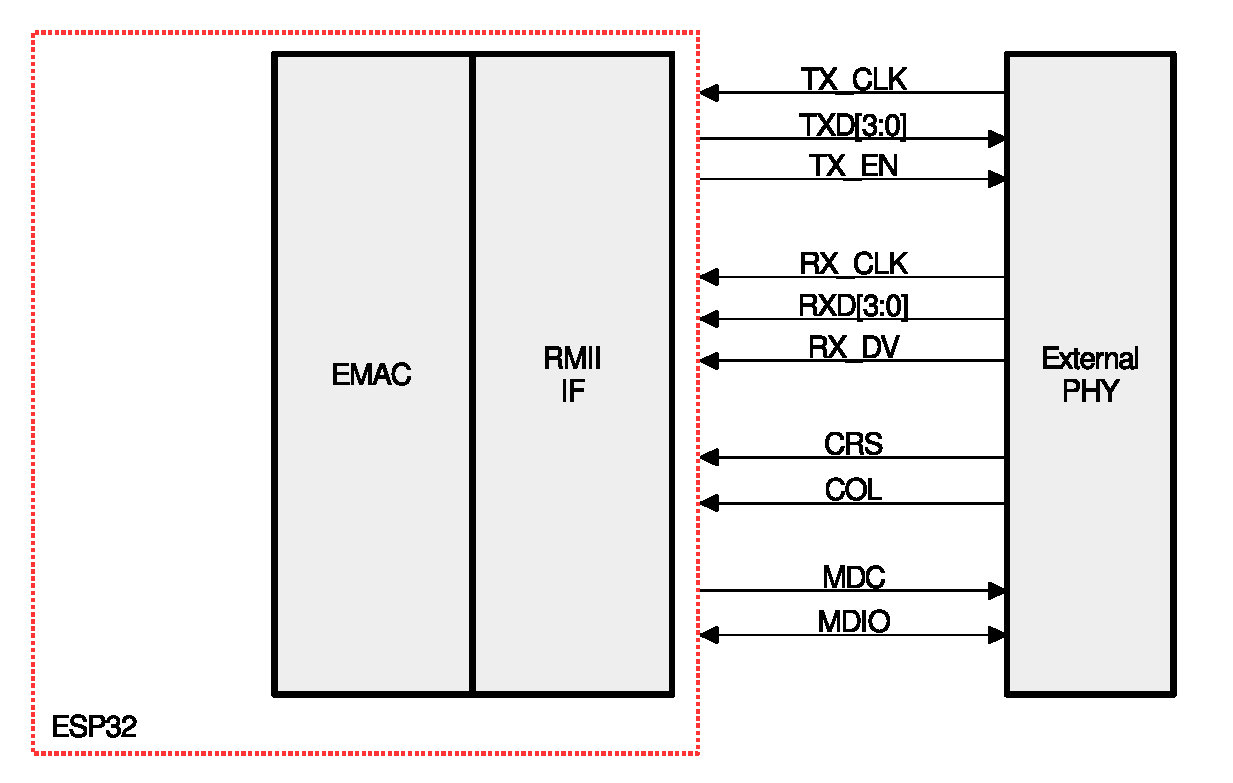
\includegraphics[width=0.6\textwidth]{./24-ETHERNETMAC/figures/Mii_IF}
    \caption{MII 接口}
    \label{Figure:Mii_IF}
\end{figure}

MII 接口信号说明：
\begin{itemize}
    \item MII\_TX\_CLK：Tx 时钟信号。该信号提供进行 Tx 数据传输时的参考时序。频率分为两种：速率为 10 Mbit/s 时为 2.5 MHz；速率为 100 Mbit/s 时为 25 MHz。
    \item MII\_TXD[3:0]：发送数据信号。该信号是 4 个一组的数据信号，由 MAC 子层同步驱动，在 MII\_TX\_EN 信号有效时才为有效信号（有效数据）。MII\_TXD[0] 为最低有效位，MII\_TXD[3] 为最高有效位。MII\_TX\_EN 信号为低时，发送数据不会对 PHY 产生任何影响。
    \item MII\_TX\_EN：发送数据使能信号。该信号表示 MAC 当前正针对 MII 发送半字节 (4 bits)。该信号必须与报头的前半字节进行同步 (MII\_TX\_CLK)，并在所有待发送的半字节均发送到 MII 时必须保持同步。
    \item MII\_RX\_CLK：RX 时钟信号。该信号提供进行 RX 数据传输时的参考时序。频率也分为两种：速率为 10 Mbit/s 时为 2.5 MHz；速率为 100 Mbit/s 时为 25 MHz。
    \item MII\_RXD[3:0]：接收数据信号。该信号是 4 个一组的数据信号，由 PHY 同步驱动，在 MII\_RX\_DV 信号有效时才为有效信号（有效数据）。MII\_RXD[0] 为最低有效位，MII\_RXD[3] 为最高有效位。当 MII\_RX\_DV 禁止、MII\_RX\_ER 使能时，特定的 MII\_RXD[3:0] 值用于代表来自 PHY 的特定信息。
    \item MII\_RX\_DV：接收数据有效信号。该信号表示 PHY 当前正针对 MII 接收已恢复并解码的半字节。该信号必须与恢复帧的头半字节进行同步于 MII\_RX\_CLK，并且一直保持同步到恢复帧的最后半字节。该信号必须在最后半字节随后的第一个时钟周期之前禁止。为了正确地接收帧，MII\_RX\_DV 信号必须在时间范围上涵盖要 接收的帧，其开始时间不得迟于 SFD 字段出现的时间。
    \item MII\_CRS：载波侦听信号。当发送或接收介质处于非空闲状态时，由 PHY 使能该信号。发送和接收介质均处于空闲状态时，由 PHY 禁止该信号。PHY 必须确保 MII\_CS 信号在冲突条件下保持有效状态。该信号无需与 Tx 和 Rx 时钟保持同步。在全双工模式下，该信号没意义。
    \item MII\_COL：冲突检测信号。检测到介质上存在冲突后，PHY 必须立即使能冲突检测 信号，并且只要存在冲突条件，冲突检测信号必须保持有效状态。该信号无需与 Tx 和 Rx 时钟保持同步。在全双工模式下，该信号没意义。
    \item MII\_RX\_ER：接收错误信号。该信号必须保持一个或多个周期 (MII\_RX\_CLK)，从而向 MAC 子层指示在帧的某处检测到错误。
    \item MDIO 和 MDC： 管理数据输入输出模块和管理数据时钟。这两个信号构成了符合 IEEE 802.3 标准的以太网串行总线，用于将控制和数据信息传输到PHY。详见 \hyperref[section:Station Management Agent (SMA) Interface]{Station Management Agent (SMA) Interface}。
\end{itemize}

\subsubsection{MII 时钟}
在 MII 时钟模式下，MII 与 PHY 的接口有 Tx 和 Rx 两个方向的时钟，MII\_TX\_CLK 用于同步 Tx 的数据，MII\_RX\_CLK 用于同步 Rx 的数据。其中 MII\_RX\_CLK 时钟由 PHY 提供，MII\_TX\_CLK 由芯片内部的 PLL 提供或是芯片外部的晶振提供。图 \ref{Figure:Mii_Clk} 的配置具体参考\hyperref[section:Ethernet Mac Register Summary]{寄存器列表}中时钟相关的寄存器。

\begin{figure}[H]
    \centering
    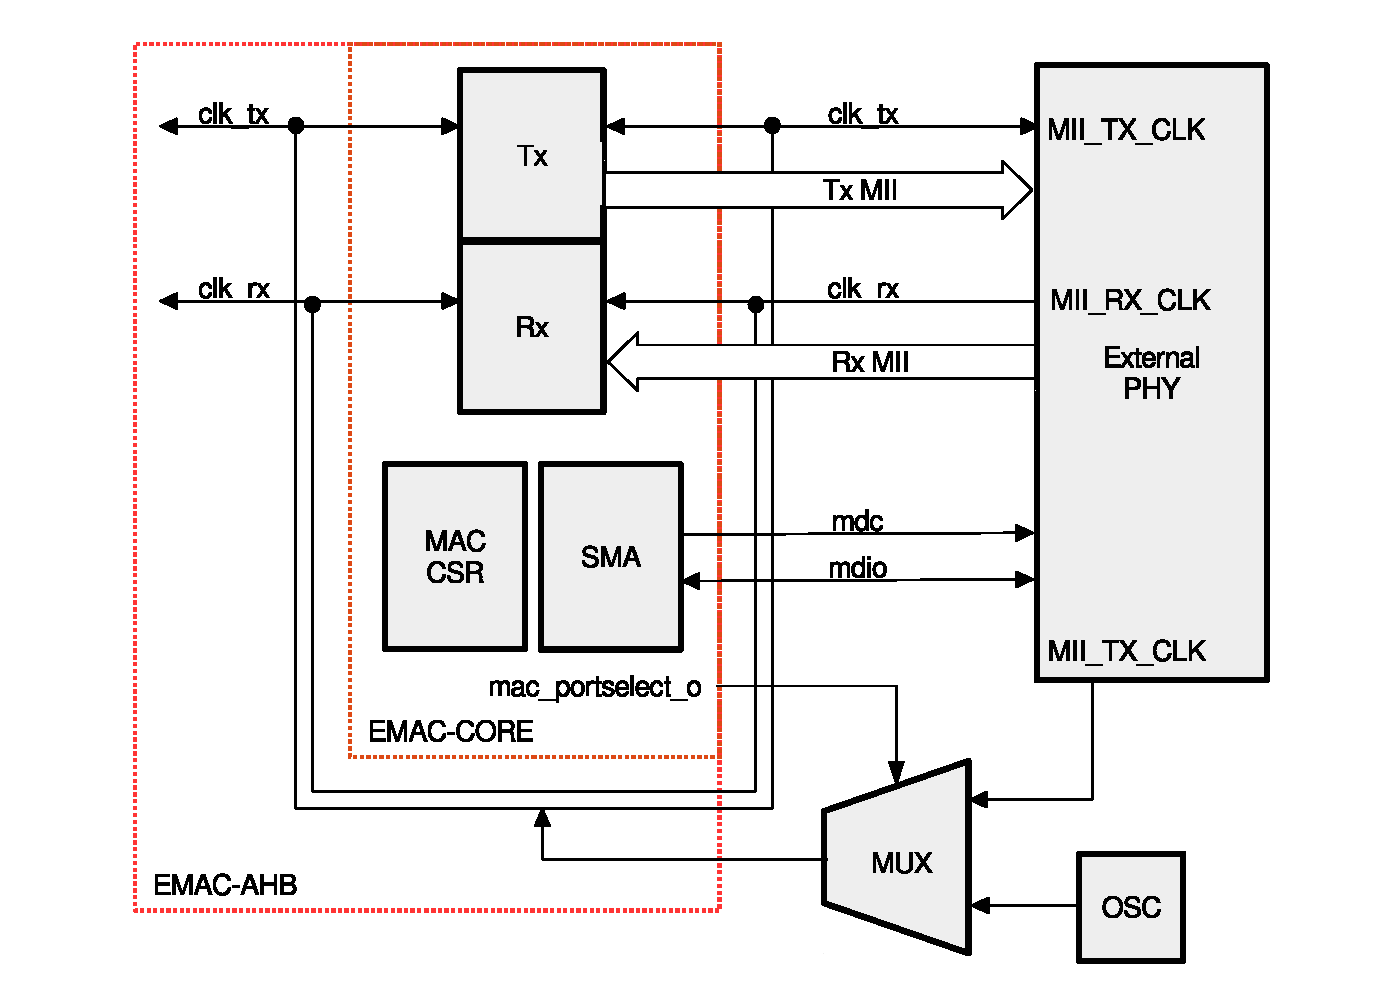
\includegraphics[width=0.8\textwidth]{./24-ETHERNETMAC/figures/Mii_Clk}
    \caption{MII 时钟}
    \label{Figure:Mii_Clk}
\end{figure}
\subsection{RMII（精简介质独立接口）}
RMII 接口信号如图 \ref{Figure:RMii_IF} 所示。\\

\begin{figure}[H]
    \centering
    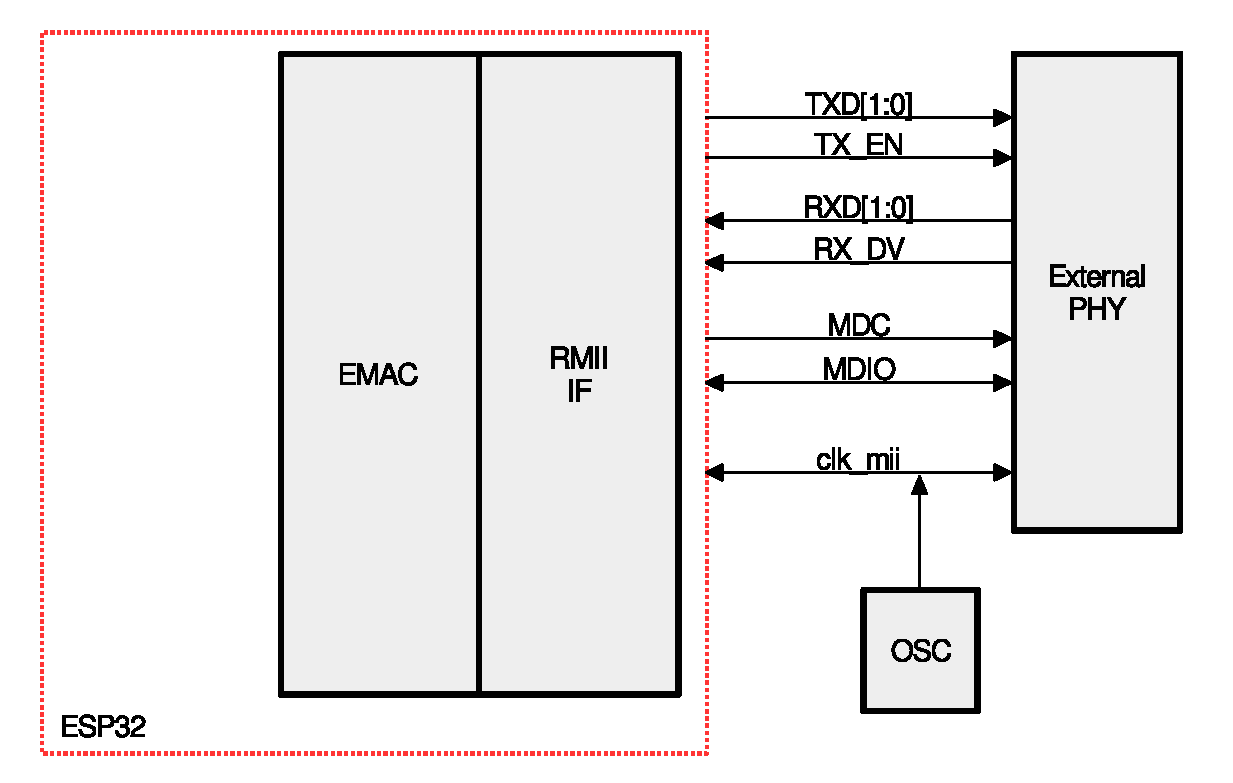
\includegraphics[width=0.7\textwidth]{./24-ETHERNETMAC/figures/RMii_IF}
    \caption{RMII 接口}
    \label{Figure:RMii_IF}
\end{figure}

\subsubsection{RMII 接口信号描述}\label{emac-rmii-interface-signal}
精简介质独立接口 (RMII) 规范降低了 10 Mbit/s 或 100 Mbit/s 下微控制器以太网外设与外部 PHY 间的引脚数。根据 IEEE 802.3u 标准，MII 包括 16 个包含数据和控制信号的引脚。RMII 规范将引脚数减少为 7 个（引脚数减少 62.5\%）。

RMII 具有以下特性：
\begin{itemize}
\item 支持 10 Mbit/s 和 100 Mbit/s 的运行速率
\item 参考时钟频率必须是 50 MHz
\item 必须提供给 MAC 和外部以太网 PHY 相同的参考时钟。PHY 提供了独立的 2 位宽的发送和接收数据的路径。
\item 请注意，如果要同时使用以太网和 Wi-Fi，则必须使用外部以太网 PHY 或外部时钟源提供 50 MHz 参考时钟。使用 ESP32 APLL 生成参考时钟会导致时钟不稳定。
\end{itemize}

\subsubsection{RMII 时钟}
RMII 时钟如图 \ref{Figure:RMii_Clk} 所示。

\begin{figure}[H]
    \centering
    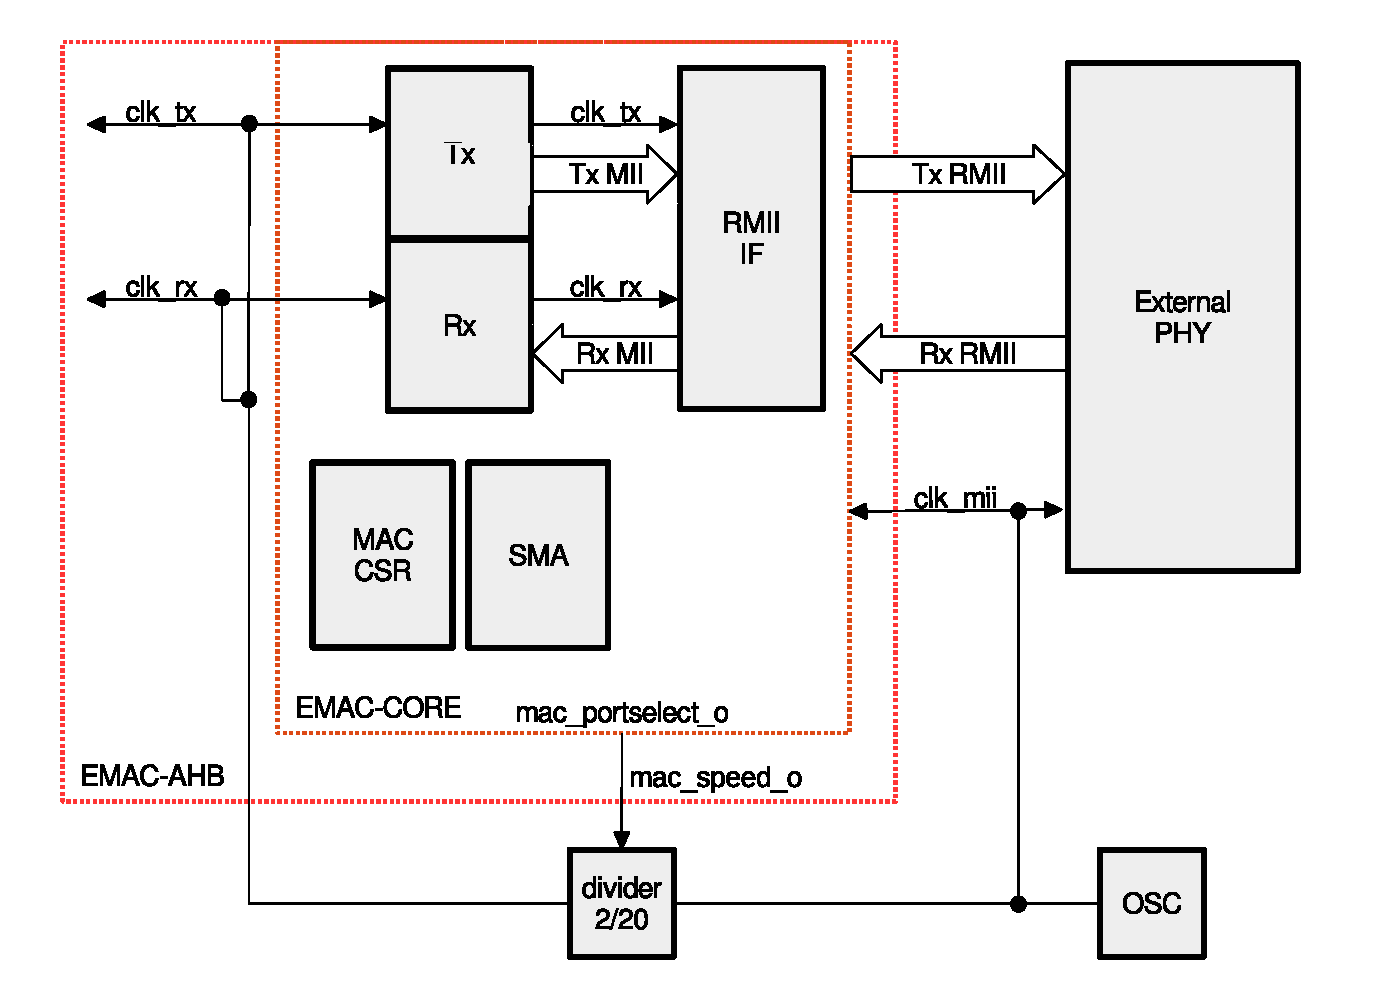
\includegraphics[width=0.8\textwidth]{./24-ETHERNETMAC/figures/RMii_Clk}
    \caption{RMII 时钟}
    \label{Figure:RMii_Clk}
\end{figure}

\subsection{Station Management Agent (SMA) 接口}
\label{section:Station Management Agent (SMA) Interface}
如图 \ref{Figure:Mii_Clk} 所示，MAC 通过 MDC 和 MDIO 信号将控制和数据信息传输到 PHY。最大时钟频率为 2.5 MHz。时钟由应用时钟通过时钟分频器分频产生。在通过 MDIO 的写/读操作期间，PHY 发送寄存器数据。该信号与 MDC 时钟同步驱动。

EMII 地址寄存器和 EMII 数据寄存器详见\hyperref[section:Ethernet Mac Register Summary]{寄存器列表}。

%%%%%%%%%%%%%%%%%%
%%%%%%%%%%%%%%%%%%

\subsection{RMII 接口时序要求}\label{section:PHY_Timing}
本章节详细说明了 RMII 接口的时序要求。
\begin{figure}[H]
    \centering
    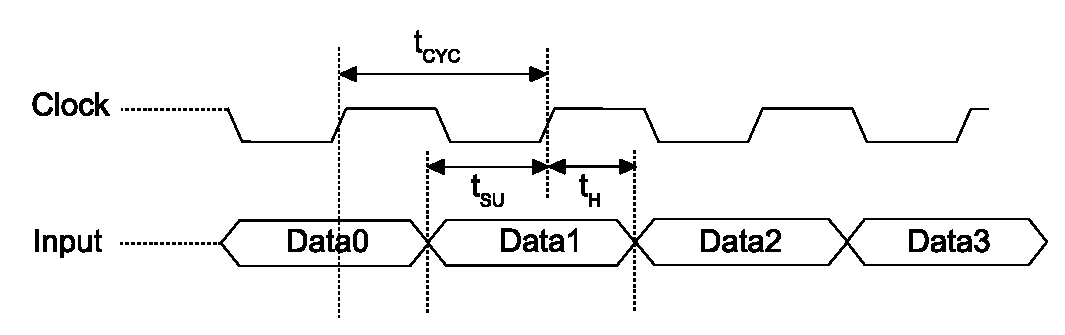
\includegraphics[width=0.6\textwidth]{./24-ETHERNETMAC/figures/ethmac_phy_timing_rx}
    \caption{接收数据时序图}
    \label{ethmac_phy_timing_rx}
\end{figure}

\begin{longtable}[c]{ | l | c | r |r|r|l| }
    \caption{接收数据时序要求}
   \\\hline

    \rowcolor{lightgray}
    \textbf{时序参数} & \textbf{描述} & \textbf{最小值} & \textbf{典型值} & \textbf{最大值} & \textbf{单位} \\\hline
    \endfirsthead
    \rowcolor{lightgray}
   \textbf{时序参数} & \textbf{描述} & \textbf{最小值} & \textbf{典型值} & \textbf{最大值} & \textbf{单位} \\\hline
    \endhead
    \endfoot
    \endlastfoot
t$_{CYC}$ & 时钟周期 (Clock cycle) & 20 & 20 & 20 & ns \\\hline
t$_{SU}$ &  建立时间 (Setup time) & 4 & – & – & ns \\\hline
t$_{H}$ & 保持时间 (Hold time) & 1 & – & – & ns \\\hline
t$_{ID}$ & 输入延迟 (Input delay) & 3 & 5 & 8 & ns \\\hline

\end{longtable}

\begin{figure}[H]
    \centering
    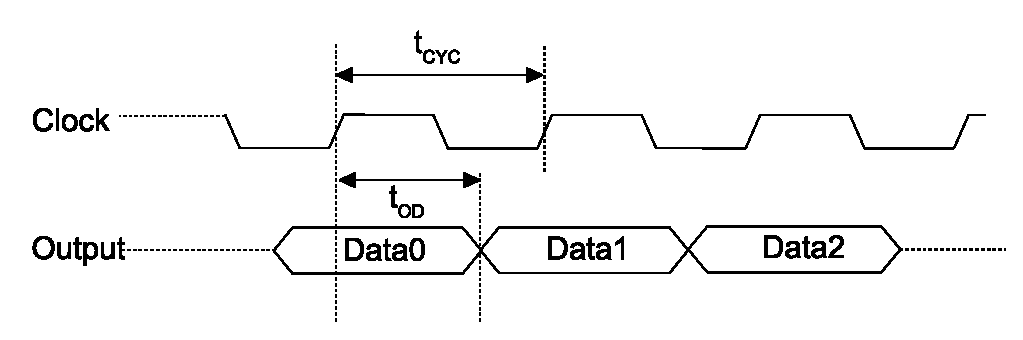
\includegraphics[width=0.6\textwidth]{./24-ETHERNETMAC/figures/ethmac_phy_timing_tx}
    \caption{发送数据时序图}
    \label{ethmac_phy_timing_tx}
\end{figure}

\begin{longtable}[c]{ | l | c | r |r|r|l| }
    \caption{发送数据时序要求}
   \\\hline

    \rowcolor{lightgray}
    \textbf{时序参数} & \textbf{描述} & \textbf{最小值} & \textbf{典型值} & \textbf{最大值} & \textbf{单位} \\\hline
    \endfirsthead
    \rowcolor{lightgray}
   \textbf{时序参数} & \textbf{描述} & \textbf{最小值} & \textbf{典型值} & \textbf{最大值} & \textbf{单位} \\\hline
    \endhead
    \endfoot
    \endlastfoot
t$_{CYC}$ & 时钟周期 (Clock cycle)  & 20 & 20 & 20 & ns \\\hline
t$_{SU}$ &  建立时间 (Setup time) & 4 & – & – & ns \\\hline
t$_{H}$ & 保持时间 (Hold time) & 1 & – & – & ns \\\hline
t$_{OD}$  & 输出延迟 (Output delay) & 6 & 9 & 12 & ns \\\hline

\end{longtable}



\section{以太网 DMA 特性}
DMA 具有独立的发送和接收引擎以及控制和状态寄存器地址。传输引擎将数据从系统内存传输到设备端口 (MTL)，而接收引擎将数据从设备端口传输到系统内存。控制器使用描述符，以最少的主机 CPU 干预来有效地将数据从源移动到目的地。DMA 用于以数据包为主的数据传输，如以太网中的帧。控制器可以配置为在正常情况下发中断给主 CPU，例如完成帧发送或接收，或发生错误时。

\section{链表描述符}
\label{section:Linked List Descriptors}
 本节介绍链表和描述符结构。每个链表由 8 个 word 组成。

\subsection{发送描述符}
发送链表结构如图 \ref{Figure:Tx_Descriptor} 所示。表 \ref{Table:TDES0} 至表 \ref{Table:TDES3} 为链表描述符说明。

\begin{figure}[H]
    \centering
    \begin{bytefield}[bitwidth=1.2em, boxformatting={\centering\small}, leftcurly=., leftcurlyspace=0pt]{32}
        \bitheader[bitformatting={\scriptsize}]{0,31} \\
        \begin{leftwordgroup}{\small \hyperref[Table:TDES0]{TDES0}}
            \bitbox{1}{\rotatebox{90}{\scriptsize OWN}} & \bitbox{5}{Ctrl[30:26]} & \bitbox{1}{\rotatebox{90}{\scriptsize Res}} & \bitbox{7}{Ctrl[24:18]} & \bitbox{1}{\rotatebox{90}{\scriptsize Res}} & \bitbox{10}{Status[16:7]} & \bitbox{4}{\scriptsize Ctrl/status \\ \scriptsize [6:3]} & \bitbox{3}{\scriptsize Status  \\ \scriptsize [2:0]}
        \end{leftwordgroup} \\
        \begin{leftwordgroup}{\small \hyperref[Table:TDES1]{TDES1}}
            \bitbox{3}{\scriptsize Ctrl \\ \scriptsize [31:29]} & \bitbox{16}{Reserved} & \bitbox{13}{Transmit Buffer Size[12:0]}
        \end{leftwordgroup} \\
        \begin{leftwordgroup}{\small \hyperref[Table:TDES2]{TDES2}}
            \bitbox{32}{Buffer Address [31:0]}
        \end{leftwordgroup} \\
        \begin{leftwordgroup}{\small \hyperref[Table:TDES3]{TDES3}}
            \bitbox{32}{Next Descriptor Address[31:0]}
        \end{leftwordgroup} \\
        \begin{leftwordgroup}{\small TDES4}
            \bitbox{32}{Reserved}
        \end{leftwordgroup} \\
        \begin{leftwordgroup}{\small TDES5}
            \bitbox{32}{Reserved}
        \end{leftwordgroup} \\
        \begin{leftwordgroup}{\small TDES6}
            \bitbox{32}{Reserved}
        \end{leftwordgroup} \\
        \begin{leftwordgroup}{\small TDES7}
            \bitbox{32}{Reserved}
        \end{leftwordgroup}
    \end{bytefield}
    \caption{发送描述符}
    \label{Figure:Tx_Descriptor}
\end{figure}

\begin{longtable}[c]{|p{1cm}|p{4cm}|p{10cm}|}
\caption{发送描述符 0 (TDES0)} \label{Table:TDES0}\\\hline
\rowcolor{lightgray}
位 &命名 & 描述 \\\hline
\endfirsthead
\hline
\rowcolor{lightgray}
位 &命名 & 描述  \\\hline
\endhead
\endfoot

\multirow{5}*{[31]}&
\multirow{5}*{OWN: Own Bit}&
该位置 1 时，表示描述符由 DMA 拥有。复位时，表示描述符由主机拥有。当 DMA 完成帧传输或分配在描述符中的缓存为空时，DMA 将清除该位。 在设置属于同一帧的所有后续描述符之后，应设置帧的第一个描述符的控制位。这避免了在获取描述符和驱动程序设置控制位之间的可能发生的竞争。\\\hline

\multirow{2}*{[30]}&
\multirow{2}*{IC: Interrupt on Completion}&
置 1 后，该位在发送当前帧之后设置发送中断 (Operation Mode Register[0])。该位仅在位 TDES0 [29] 置 1 时有效。
\\\hline

\multirow{2}*{[29]}&
\multirow{2}*{LS: Last Segment}&
置 1 时，该位表示缓存区中包含该帧的最后一段。当该位置 1 时，TDES1 中的 TBS1 或 TBS2 字段的值不为零。\\\hline
[28]&
FS: First Segment&
置 1 时，该位表示缓存区中包含帧的第一段。\\\hline

\multirow{2}*{[27]}&
\multirow{2}*{DC: Disable CRC}&
该位置 1 时，MAC 不会在发送帧的末尾附加循环冗余校验 (CRC)。这仅在位 TDES0 [28] 置 1 时有效。
\\\hline
\multirow{4}*{[26]}&
\multirow{4}*{DP: Disable Pad}&
置 1 时，MAC 不会自动在短于 64 字节的帧后面自动添加 padding。当该位复位时，DMA 自动将 padding 和 CRC 添加到短于 64 个字节的帧中，并且无论 DC (TDES0 [27]) 位的状态如何，都会添加 CRC 字段。只有当位 TDES0 [28] 置 1 时才有效。\\\hline

[25]& Reserved & 保留\\\hline

\multirow{4}*{[24]}&
\multirow{4}*{\makecell[l]{CRCR: CRC Replacement\\Control}}&
 置 1 时，MAC 用重新计算的 CRC 字节替换发送的数据包的最后四个字节。主机应确保 CRC 字节在将要发送的帧的缓存中。当控制位 (TDES0 [28]) 置 1 时，该位有效。另外，只有当位 TDES0 [27] 置 1 时才进行 CRC 替换。\\\hline

\multirow{8}*{[23:22]}&\multirow{8}*{
\makecell[l]{CIC: Checksum Insertion\\Control}}&
 这些位控制校验和的计算和插入。以下列表描述了位编码：
\begin{itemize}
\item 2'b00：关闭校验和插入。
\item 2'b01：仅使能 IP 报头校验和计算和插入。
\item 2'b10：使能 IP 报头校验和以及有效负载校验的计算和插入，伪报头校验不在硬件中计算。
\item 2'b11：使能 IP 报头校验和以及有效负载校验的计算和插入，但是伪报头校验在硬件中计算。
\end{itemize}
当控制位 TDES0 [28] 置 1 时，此字段有效。\\\hline

\multirow{2}*{[21]}&
\multirow{2}*{TER: Transmit End of Ring}&
置 1 时，该位表示描述符列表已达到最后一个链表描述符。DMA 返回到链表的基地址，创建一个描述符环。\\\hline

\multirow{3}*{[20]}&
\multirow{3}*{\makecell[l]{TCH: Second Address\\Chained}} &
置 1 时，该位指示描述符中的第二个地址是下一个描述符地址。当 TDES0 [20] 置 1 时，TBS2 (TDES1 [28:16]) 是一个“无关”值。TDES0 [21] 优先于 TDES0 [20]。此位必须置 1。\\\hline

\multirow{9}*{[19:18]}&
\multirow{9}*{\makecell[l]{VLIC: VLAN Insertion\\Control}}&
置 1 时，这些位请求 MAC 在传输帧之前打上 VLAN 标记或取消标记。如果帧被打上 VLAN 标记，则 MAC 会自动重新计算并替换 CRC 字节。以下为这些位的说明：
\begin{itemize}
\item 2'b00：不加上 VLAN 标记。
\item 2'b01：在传输之前去掉 VLAN 标记，只用于 VLAN 帧。
\item 2'b10：插入 VLAN 标记，标记的值在 VLAN 标记插入和替换寄存器中配置。
\item 2'b11：用 VLAN 标记插入和替换寄存器中的标记值替换帧当中的 VLAN 标记。该选项只能用于 VLAN 帧。\vspace{-1.5em}
\end{itemize}\\\hline

[17]& Reserved & 保留\\\hline

\multirow{6}*{[16]}&
\multirow{6}*{IHE: IP Header Error}&
置 1 时，该位指示 MAC 发送器在 IP 报头中检测到错误。发送器检查 IPv4 数据包中的报头长度与从应用程序接收到的报头字节的数量，如果不匹配，则指示错误状态。对于 IPv6 帧，如果报头长度不是 40 个字节，则指示报头错误。此外，IPv4 或 IPv6 帧的“以太网长度/类型”字段值必须与接收到的 IP 报头版本匹配。对于 IPv4 帧，如果“报头长度”字段的值小于 0x5，则指示错误状态。
\\\hline

\multirow{11}*{[15]}&
\multirow{11}*{ES: Error Summary}&
此位代表以下 bit 的逻辑或:
\begin{itemize}
\item TDES0[14]: Jabber 超时
\item TDES0[13]: 帧刷新
\item TDES0[11]: 载波丢失
\item TDES0[10]: 无载波
\item TDES0[9]: 延迟冲突
\item TDES0[8]: 过度冲突
\item TDES0[2]: 过度延迟
\item TDES0[1]: 下溢错误
\item TDES0[16]: IP 报头错误
\item TDES0[12]: IP 有效负载错误
\vspace{-1.5em}\end{itemize}
\\ \hline
\multirow{2}*{[14]}&
\multirow{2}*{JT: Jabber Timeout}&
置 1 时，该位表示 MAC 发送器发生了 jabber 超时。只有在 EMACCONFIG\_REG 的 EMACJABBER 位（关闭 Jabber）未置 1 时，该位置 1。\\\hline
\multirow{2}*{[13]}&
\multirow{2}*{FF: Frame Flushed}&
置 1 时，该位表示 DMA 或 MTL 已经按照 CPU 给出的刷新命令刷新帧。\\\hline
\multirow{5}*{[12]}&
\multirow{5}*{IPE: IP Payload Error}&
置 1 时，该位表示 MAC 发送器在 TCP，UDP 或 ICMP IP 数据报有效载荷中检测到错误。\\
& & 发送器检查 IPv4 或 IPv6 报头中收到的有效负载长度与从应用程序接收到的 TCP，UDP 或 ICMP 数据包字节的实际数量，并在发生不匹配时指示错误状态。\\\hline
\multirow{3}*{[11]}&
\multirow{3}*{LOC: Loss of Carrier}&
置 1 时，该位指示在帧传输期间发生载波丢失（即，在帧传输期间，一个或多个传输时钟周期内，MII\_CRS 信号无效）。当 MAC 处于半双工模式时，只对传输中没有冲突的帧有效。\\\hline
\multirow{2}*{[10]}&
\multirow{2}*{NC: No Carrier}&
置 1 时，该位指示在传输过程中来自 PHY 的载波侦听信号未被拉低。\\\hline
\multirow{3}*{[9]}&
\multirow{3}*{LC: Late Collision}&
置 1 时，该位指示由于冲突窗口（在 MII 模式下，包括报头在内共 64 字节时间，和 512 字节时间，包括报头和载波扩展）之后发生冲突而发生的帧传输被中止。如果下溢错误位置 1，则该位无效。\\\hline
\multirow{3}*{[8]}&
\multirow{3}*{EC: Excessive Collision}&
置 1 时，该位表示在尝试传送当前帧发生 16 次连续冲突之后传输被中止。如果 EMACCONFIG\_REG 的 EMACRETRY 位置 1，则该位在第一次冲突后置 1，并且帧传输被中止。\\\hline
[7]&
VF: VLAN Frame&
置 1 时，表示传输的帧是 VLAN 类型的帧。\\\hline
\multirow{3}*{[6:3]}&
\multirow{3}*{\makecell[l]{Ctrl/status}}&
 这些状态位指示帧发送之前发生的冲突次数。当过度冲突位 (TDES0 [8]) 置 1 时，此计数无效。CPU 只在半双工模式下更新这个状态字段。\\\hline
\multirow{3}*{[2]}&
\multirow{3}*{ED: Excessive Deferral}&
置 1 时，如果 MAC 配置寄存器 EMACCONFIG\_REG 的 EMACDEFERRALCHECK（延迟检测）位置为高，则该位表示传输已经结束，原因是在使能巨帧的情况下，过度延迟超过 24,288 比特时间。\\\hline
\multirow{4}*{[1]}&
\multirow{4}*{UF: Underflow Error}&
置 1 时，该位表示由于数据从主机存储器延迟到达，MAC 中止了帧发送。下溢错误表示 DMA 在传输帧时遇到空的传输缓存。传输过程进入暂停状态并将传输下溢寄存器（状态寄存器 bit[5]） 和传输中断寄存器（状态寄存器 bit[0]）置 1。
\\\hline
\multirow{2}*{[0]}&
\multirow{2}*{DB: Deferred Bit}&
置 1 时，该位表示 MAC 由于载波的存在而传输延迟。该位仅在半双工模式下有效。\\\hline
\end{longtable}

\begin{longtable}[c]{ |p{1cm}|p{4cm}|p{10cm}| }
\caption{发送描述符 1 (TDES1)} \label{Table:TDES1}\\
\hline
\rowcolor{lightgray}
位&名称&描述\\
\hline
\endfirsthead
\hline
\rowcolor{lightgray}
位&名称&描述 \\
\hline
\endhead
\endfoot
\multirow{12}*{[31:29]}&
\multirow{12}*{SAIC: SA Insertion Control}&
这些位请求 MAC 使用 GMACADDR0HIGH\_REG，GMACADDR0LOW\_REG，GMACADDR1HIGH\_REG，GMACADDR1HIGH\_REG 寄存器中给定的值添加或替换以太网帧中的源地址字段。如果“源地址”字段在帧中被修改，则 MAC 会自动重新计算并替换 CRC 字节。位 31 指定用于插入或替换源地址的 MAC 地址寄存器值（1 或 0）。以下列表描述了位 [30:29] 的值：

\begin{itemize}
\item 2'b00：不加入源地址。
\item 2'b01：插入源地址。为确保传输的可靠性，应用程序必须提供没有源地址的帧。
\item 2'b10：替换源地址。为确保传输的可靠性，应用程序必须提供带有源地址的帧。
\item 2'b11：保留
\end{itemize}当控制位 TDES0 [28] 置 1 时，这些位有效。\\\hline
[28:16]&Reserved&保留\\\hline
[15:13]&Reserved&保留\\\hline
\multirow{2}*{[12:0]}&
\multirow{2}*{\makecell[l]{TBS1: Transmit Buffer\\Size}}&
链表数据缓存的大小，以字节为单位。如果该字段为 0，则 DMA 将忽略此缓存，并使用下一个描述符。\\\hline
\end{longtable}

\begin{longtable}[c]{ |p{1cm}|p{4cm}|p{10cm}| }
\caption{发送描述符 2 (TDES2)} \label{Table:TDES2}\\
\hline
\rowcolor{lightgray}
位&名称&描述\\
\hline
\endfirsthead
\hline
\rowcolor{lightgray}
位&名称&描述 \\\hline
\endhead
\endfoot
[31:0]& Buffer Address Pointer& 缓存的物理地址。\\\hline
\end{longtable}


\begin{longtable}[c]{ |p{1cm}|p{4cm}|p{10cm}| }
\caption{发送描述符 3 (TDES3)} \label{Table:TDES3}\\
\hline
\rowcolor{lightgray}
位 &名称 & 描述 \\
\hline
\endfirsthead
\hline
\rowcolor{lightgray}
位 &名称 & 描述  \\\hline
\endhead
\endfoot
[31:0]&Next Descriptor Address&该地址包含下一个描述符所在物理内存的指针。\\\hline
\end{longtable}


\subsection{接收描述符} 接收链表结构如图 \ref{Figure:Rx_Descriptor} 所示。表 \ref{Table:RDES0} 至表 \ref{Table:RDES4} 为链表描述。

\begin{figure*}[h!]
    \centering
    \begin{bytefield}[bitwidth=1.2em, boxformatting={\centering\small}, leftcurly=., leftcurlyspace=0pt]{32}
        \bitheader[bitformatting={\scriptsize}]{0,31} \\
        \begin{leftwordgroup}{\small \hyperref[Table:RDES0]{RDES0}}
            \bitbox{1}{\rotatebox{90}{\scriptsize OWN}} & \bitbox{31}{Status[30:0]}
        \end{leftwordgroup} \\
        \begin{leftwordgroup}{\small \hyperref[Table:RDES1]{RDES1}}
            \bitbox{1}{\rotatebox{90}{\scriptsize Ctrl}} & \bitbox{15}{Reserved[30:16]} & \bitbox{2}{\scriptsize Ctrl \\ \scriptsize [15:14]} & \bitbox{1}{\rotatebox{90}{\scriptsize Res}} & \bitbox{13}{Receive Buffer 1 Size[12:0]}
        \end{leftwordgroup} \\
        \begin{leftwordgroup}{\small \hyperref[Table:RDES2]{RDES2}}
            \bitbox{32}{Buffer1 Address [31:0]}
        \end{leftwordgroup} \\
        \begin{leftwordgroup}{\small \hyperref[Table:RDES3]{RDES3}}
            \bitbox{32}{Next Descriptor Address[31:0]}
        \end{leftwordgroup} \\
        \begin{leftwordgroup}{\small \hyperref[Table:RDES4]{RDES4}}
            \bitbox{32}{Extended Status[31:0]}
        \end{leftwordgroup} \\
        \begin{leftwordgroup}{\small RDES5}
            \bitbox{32}{Reserved}
        \end{leftwordgroup} \\
        \begin{leftwordgroup}{\small RDES6}
            \bitbox{32}{Reserved}
        \end{leftwordgroup} \\
        \begin{leftwordgroup}{\small RDES7}
            \bitbox{32}{Reserved}
        \end{leftwordgroup}
    \end{bytefield}
    \caption{接收链表结构}
    \label{Figure:Rx_Descriptor}
\end{figure*}


\label{Receive Descriptor 0}
\begin{longtable}[c]{ |p{1cm}|p{4cm}|p{10cm}| }
\caption{接收描述符 0 (RDES0)} \label{Table:RDES0}\\
\hline
\rowcolor{lightgray}
位 &名称 & 描述 \\
\hline
\endfirsthead
\hline
\rowcolor{lightgray}
位&名称&描述\\
\hline
\endhead
\endfoot


\multirow{3}*{[31]}&
\multirow{3}*{OWN: Own Bit}& 置 1 时，该位表示描述符由 DMA 所有。当该位复位时，该位表示描述符由主机拥有。DMA 在完成帧接收或与此链表有关的缓存已满时清除该位。\\
\hline
\multirow{2}*{[30]}&
AFM: Destination Address Filter Fail&
\multirow{2}*{置 1 时，该位表示 MAC 中 DA 滤波器失败的帧。}\\\hline
\multirow{4}*{[29:16]}&
\multirow{4}*{FL: Frame Length}&
这些位表示发送到 CPU 内存的接收帧的字节长度。当 RDES0 [8] 被置 1 且描述符错误位 RDES0 [14] 或溢出错误位被复位时，该字段有效。当使能 IP 校验和计算（类型 1）并且所接收的帧不是 MAC 控制帧时，帧长度还包括附加到以太网帧的两个字节。\\\hline
\multirow{10}*{[15]}&
\multirow{10}*{ES: Error Summary}& 该字段表示以下位的逻辑或：
\begin{itemize}
\item RDES0[1]：CRC 错误
\item RDES0[3]：接受错误
\item RDES0[4]：看门狗超时
\item RDES0[6]：延迟冲突
\item RDES0[7]：巨帧
\item RDES4[4:3]：IP 报头或负载错误
\item RDES0[11]：上溢错误
\item RDES0[14]：描述符错误
\end{itemize}
只有 RDES0 [8] 置 1 时，该字段有效。\\\hline

\multirow{3}*{[14]}&
\multirow{3}*{DE: Descriptor Error}&
置 1 时，该位表示由帧大小超过当前描述符缓存的帧被截断，并且 DMA 不拥有下一个描述符。该帧被截断。只有当位 RDES0 [8] 置 1 时，该字段才有效。
\\\hline
\multirow{2}*{[13]}&
SAF: Source Address Filter Fail&
\multirow{2}*{置 1 时，该位表示帧的 SA 字段未通过 MAC 中的 SA 过滤。}\\\hline
\multirow{2}*{[12]}&
\multirow{2}*{LE: Length Error}&
置 1 时，该位表示接收到的帧的实际长度和长度/类型字段不匹配。该位仅在帧类型 (RDES0 [5]) 位复位时有效。\\\hline
\multirow{2}*{[11]}&
\multirow{2}*{OE: Overflow Error}&
置 1 时，该位表示由于 MTL 中的缓存溢出而导致接收到的帧被损坏。\\\hline
\multirow{3}*{[10]}&
\multirow{3}*{VLAN: VLAN Tag}&
置 1 时，该位表示该描述符所指向的帧是由 MAC 标记的 VLAN 帧。VLAN 标记取决于根据 VLAN 标记寄存器设置检查接收到的帧的 VLAN 字段。
\\\hline
\multirow{3}*{[9]}&
\multirow{3}*{FS: First Descriptor}&
置 1 时，该位表示该描述符包含帧的第一个缓存区。如果第一个缓存区的大小是 0，则该帧从第二个缓存开始。如果第二个缓存的大小也是 0，则下一个描述符包含该帧的帧头。\\\hline
[8]&
LS: Last Descriptor&
置 1 时，该位表示该描述符指向的缓存是该帧的最后一个缓存区。\\\hline
\multirow{13}*{[7]}&
\multirow{13}*{\makecell[l]{IP Checksum Error (Type1),\\or Giant Frame}}&

当选择 IP 校验和引擎（类型 1）时，该位置 1 表示以下情况之一：
\begin{itemize}
\item  MAC 内核计算的 16 位 IPv4 报头校验和与收到的校验和字节不匹配。
\item 非 IPv4 帧绕过报头校验和检查。
\end{itemize}
若以上两种情况都不符合，则该位置 1 表示巨帧状态。对于普通帧，大于 1,518 字节的帧为巨帧（若该普通帧为 VLAN 帧，则大于 1,522 字节的帧为巨帧；当 GMAC\_CONFIGREG bit[27] 为 1 时，大于 2,000 字节的帧为巨帧）。当使能巨帧处理时，大于 9,018 字节的帧为巨帧（若该巨帧为 VLAN 帧，则大于 9,022 字节的帧为巨帧）。
\\\hline
[6]&
LC: Late Collision&
置 1 时，该位表示在半双工模式下接收帧时发生延迟冲突。\\\hline
\multirow{3}*{[5]}&
\multirow{3}*{FT: Frame Type}&
置 1 时，该位表示接收帧是以太网类型的帧（LT 字段大于或等于 1,536 字节）。 当该位复位时，表示接收到的帧是 IEEE 802.3 帧。此位对于小于 14 个字节的矮帧无效。\\\hline
\multirow{2}*{[4]}&
\multirow{2}*{\makecell[l]{RWT: Receive\\Watchdog Timeout}}&
置 1 表示接收看门狗定时器在收到当前帧时已经超时，当前帧在看门狗超时后被截断。\\\hline
\multirow{2}*{[3]}&
\multirow{2}*{RE: Receive Error}&
置 1 时，该位表示在接收帧期间若 MII\_RXDV 被置 1，则发出 MII\_RXER。\\\hline
\multirow{2}*{[2]}&
\multirow{2}*{DE: Dribble Bit Error}&置 1 时，该位表示接收到的帧具有非整数倍的字节（奇数个半字节）。该位仅在 MII 模式下有效。\\\hline
\multirow{2}*{[1]}&
\multirow{2}*{CE: CRC Error}&
置 1 时，该位表示在接收到的帧上发生循环冗余校验 (CRC) 错误。只有位 RDES0 [8] 置 1 时，该字段才有效。\\\hline
\multirow{10}*{[0]}&
\multirow{10}*{\makecell[l]{Extended Status Available/\\Rx MAC Address}}&
当 IP 校验和卸载（类型 2）存在时，该位置 1 时表明扩展状态在描述符字 4 (RDES4) 中可用。 只有位 RDES0 [8] 置 1 时才有效。位 30 置 1 时该位无效。\\
& & 当 IP 校验和卸载（类型 2）存在时，即使在 IP 校验和卸载引擎绕过接收帧的处理，该位也被置 1。绕过可能是因为非 IP 帧或非 TCP/UDP/ICMP 有效载荷的 IP 帧。\\
& &
当 IPC 全部卸载未被选择时，该位表示 Rx MAC 地址状态。置 1 时，该位表示 Rx MAC 地址寄存器值（1 至 15）与帧的 DA 字段相匹配。复位时，该位表示 Rx MAC 地址寄存器 0 的值与 DA 字段匹配。\\\hline

\end{longtable}


\begin{longtable}[c]{ |p{1cm}|p{4cm}|p{10cm}| }
\caption{接收描述符 1 (RDES1)} \label{Table:RDES1}\\
\hline
\rowcolor{lightgray}
位&名称&描述\\
\hline
\endfirsthead
\hline
\rowcolor{lightgray}
位&名称&描述 \\
\hline
\endhead
\endfoot
\multirow{3}*{[31]}&
\multirow{3}*{\makecell[l]{Ctrl}}&
置 1 时，该位阻止帧的状态寄存器的 RI 位 (CSR5 [6]) 被置 1，使得收到的帧在当前描述符所指的缓存内结束。从而禁止由于该帧的 RI 向主机的中断触发。
\\\hline
[30:29]&Reserved&保留\\\hline
[28:16]&Reserved&保留\\\hline
\multirow{2}*{[15]}&
\multirow{2}*{RER: Receive End of Ring}&
置 1 时，该位表示描述符列表已达到其最后一个描述符。DMA 返回到列表的基地址，创建一个描述符环。\\\hline
\multirow{3}*{[14]}&
\multirow{3}*{\makecell[l]{RCH: Second Address\\Chained}}&
置 1 时，该位表示描述符中的第二个地址是下一个描述符地址，此位必须置 1。当该位置 1 时，RBS2 (RDES1 [28:16]) 是一个“无关”值。 RDES1 [15] 优先级高于 RDES1 [14]。\\\hline
[13]&
Reserved&
保留\\\hline
\multirow{4}*{[12:0]}&
\multirow{4}*{\makecell[l]{RBS1: Receive Buffer 1\\Size}}&
表示第一个数据缓存的大小（字节）。即使 RDES2（buffer1 地址指针）的值未对齐，缓存大小也必须是 4 的倍数。当缓存大小不是 4 的倍数时，结果是不确定的。如果该字段为 0，则 DMA 将忽略此缓存，并根据 RCH 的值 (bit[14]) 使用缓存 2 或下一个描述符。\\\hline

\end{longtable}


\begin{longtable}[c]{ |p{1cm}|p{4cm}|p{10cm}| }
\caption{接收描述符 2 (RDES2)} \label{Table:RDES2}\\
\hline
\rowcolor{lightgray}
位&名称&描述\\
\hline
\endfirsthead
\hline
\rowcolor{lightgray}
位&名称&描述 \\
\hline
\endhead
\endfoot
[31:0]&
Buffer Address Pointer&
这些位表示缓存的物理地址。\\\hline

\end{longtable}


\begin{longtable}[c]{ |p{1cm}|p{4cm}|p{10cm}| }
\caption{接收描述符 3 (RDES3)} \label{Table:RDES3}\\
\hline
\rowcolor{lightgray}
位&名称&描述\\
\hline
\endfirsthead
\hline
\rowcolor{lightgray}
位&名称&描述 \\\hline
\endhead
\endfoot
[31:0]&Next Descriptor Address&该地址包含指向下一个描述符所在物理内存的指针。\\\hline
\end{longtable}


\begin{longtable}[c]{ |p{1cm}|p{4cm}|p{10cm}| }
\caption{接收描述符 4 (RDES4)} \label{Table:RDES4}\\
\hline
\rowcolor{lightgray}
位&名称&描述\\
\hline
\endfirsthead
\hline
\rowcolor{lightgray}
位&名称&描述 \\
\hline
\endhead
\endfoot
[31:28]&
Reserved&
保留\\\hline
[27:26]&
Reserved&
保留 \\\hline
[25]&
Reserved&
保留\\\hline
[24]&
Reserved&
保留\\\hline
[23:21]&
Reserved&
保留\\\hline
[20:18]&
Reserved&
保留\\\hline
[17]&
Reserved&
保留 \\\hline
[16]&
Reserved&
保留 \\\hline
[15]&
Reserved&
保留\\\hline
[14]&
Reserved&
保留\\\hline
[13]&
Reserved&
保留\\\hline
[12]&
Reserved&
保留\\\hline
\multirow{14}*{[11:8]}&\multirow{14}*{
Message Type} &
这些位被编码成所接收消息的类型。
\begin{itemize}
\item 3'b0000：保留
\item 3'b0001：SYNC (所有时钟类型)
\item 3'b0010：Follow\_Up (所有时钟类型)
\item 3'b0011：Delay\_Req (所有时钟类型)
\item 3'b0100：Delay\_Resp (所有时钟类型)
\item 3'b0101：Pdelay\_Req (点对点透明时钟)
\item 3'b0110：Pdelay\_Resp (点对点透明时钟)
\item 3'b0111：Pdelay\_Resp\_Follow\_Up (点对点透明时钟)
\item 3'b1000：Announce
\item 3'b1001：Management
\item 3'b1010：Signaling
\item 3'b1011-3'b1110：保留
\item 3'b1111：保留
\vspace{-1.5em} \end{itemize}
\\ \hline
\multirow{2}*{[7]}&
\multirow{2}*{IPv6 Packet Received}&
置 1 时，该位表示接收到的数据包是一个 IPv6 数据包。该位仅在寄存器（MAC 配置寄存器）的 bit[10] (IPC) 置 1 时更新。\\\hline
\multirow{2}*{[6]}&
\multirow{2}*{IPv4 Packet Received}&
 置 1 时，表示接收到的数据包是 IPv4 数据包。该位仅在寄存器（MAC 配置寄存器）的 bit[10] (IPC) 置 1 时更新。\\\hline
[5]&
IP Checksum Bypassed&
置 1 时，该位表示校验和卸载引擎被旁路。 \\\hline
\multirow{4}*{[4]}&
\multirow{4}*{IP Payload Error}&
置 1 时，该位表示 MAC 内核计算的 16 位 IP 有效负载校验和（即 TCP，UDP 或 ICMP 校验和）与接收的段中对应的校验和字段不匹配。当 TCP，UDP 或 ICMP 段的长度与 IP Header 字段中的负载长度值不匹配时，该位置 1。当 bit[7] 或 bit[6] 置 1 时，该位有效。\\\hline
\multirow{3}*{[3]}&
\multirow{3}*{IP Header Error}&
置 1 时，该位表示由 MAC 内核计算的 16 位 IPv4 报头校验和与接收的校验和字节不匹配，或 IP 数据报版本与以太网类型值不一致。当 bit[7] 或 bit[6] 被置 1 时，该位有效。\\\hline
\multirow{10}*{[2:0]}&
\multirow{10}*{IP Payload Type}&这些位表示封装在由接收校验和卸载引擎 (COE) 处理的 IP 数据报中的有效载荷的类型。如果 COE 由于 IP 报头错误或分段 IP 而不处理 IP 数据报的有效载荷，COE 也将这些位置为 2'b00。
\begin{itemize}
\item 3'b000：未知或未处理 IP 负载
\item 3'b001：UDP
\item 3'b010：TCP
\item 3'b011：ICMP
\item 3'b1xx：保留
\end{itemize}
当位 7 或位 6 置 1 时，该位有效。\\\hline
\end{longtable}


\hypertarget{ethernetmac-reg-summ}{}
\section{寄存器列表}
\label{section:Ethernet Mac Register Summary}
 特定寄存器的特定字段或位具有不同的访问属性。以下列表为寄存器描述中使用的属性缩写。

\begin{itemize}
    \item Read Only (RO) 只读
    \item Write Only (WO) 只写
    \item Read and Write (R/W) 读/写
    \item Read, Write, and Self Clear (R/W/SC) 读/写/自动清除
    \item Read, Self Set, and Write Clear (R/SS/WC) 读/自动设置/写清除
    \item Read, Write Set, and Self Clear (R/WS/SC) 读/写设置/自动清除
    \item Read, Self Set, and Self Clear or Write Clear (R/SS/SC/WC) 读/自动设置/自动清除/写清除
    \item Read Only and Write Trigger (RO/WT) 只读/写触发
    \item Read, Self Set, and Read Clear (R/SS/RC) 读/自动设置/读清除
    \item Read, Write, and Self Update (R/W/SU)读/写/自动更新
    \item Latched-low (LL) 低锁存
    \item Latched-high (LH) 高锁存
\end{itemize}

\subfile{\modulefiles/ethernet_reg-summary_cn.tex}

\section{寄存器}\label{ethernetreg}

\textbf{说明：所有 reserved 寄存器的值必须保持复位值。}

本小节的所有地址均为相对于 EMAC 基地址的地址偏移量（相对地址），具体基地址请见章节 \ref{mod:sysmem} \textit{\nameref{mod:sysmem}} 中的表 \ref{table:Peripheral_Address_Mapping}。寄存器绝对地址见章节 \ref{sec:gpio-reg-summ} \textit{\nameref{sec:gpio-reg-summ}}。

关于保留 (reserved) 域的处理，请查看章节 \hyperref[programming-reserved-field]{\textit{如何配置寄存器的保留域}}。

\subfile{\modulefiles/ethernet_reg_cn.tex}

\end{document}
